\section{Caso para estudo} \label{sec:chap4}

Consideramos um quarto com alguns dispositivos IoT para controlar automaticamente sua temperatura e iluminação. Para isso foi configurado um conjunto de sensores, controladores e atuadores para o ar condicionado, o aquecedor e as luzes do quarto.
A rede foi configurada de forma para ligar e desligar automaticamente o ar condicionado ou o aquecedor quando a temperatura estiver muito quente ou fria, e desligá-los quando a temperatura estiver amena. As luzes ligam e desligam automaticamente baseadas na luminosidade do quarto, e ficam desligadas durante a madrugada.
A figura \ref{fig:fig2} mostra um diagrama que representa como os componentes estão conectados.
Para mais detalhes, veja o Apêndice \ref{apx:apx1}.

\begin{figure}[ht]
  \centering
  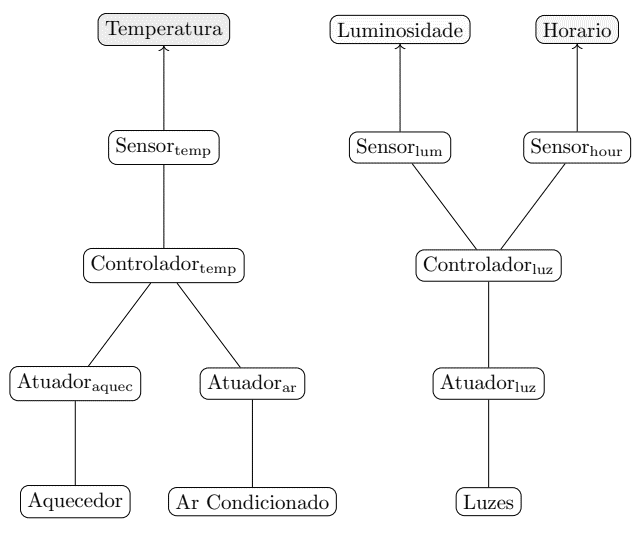
\includegraphics[width=0.5\textwidth]{img/network-diagram.png}
  \caption{Diagrama de componentes}
  \label{fig:fig2}
\end{figure}